\documentclass[a4paper, landscape, DIV=14]{scrartcl}
\usepackage[utf8]{inputenc}
\usepackage[T1]{fontenc}
\usepackage{tikz,amsmath}

% Define bright colors.
\definecolor{TolBrightBlue}{HTML}{4477AA}
\definecolor{TolBrightCyan}{HTML}{66CCEE}
\definecolor{TolBrightGreen}{HTML}{228833}
\definecolor{TolBrightYellow}{HTML}{CCBB44}
\definecolor{TolBrightRed}{HTML}{EE6677}
\definecolor{TolBrightPurple}{HTML}{AA3377}
\definecolor{TolBrightGray}{HTML}{BBBBBB}

\definecolor{TolMutedBlue}{HTML}{332288}
\definecolor{TolMutedCyan}{HTML}{88CCEE}
\definecolor{TolMutedTeal}{HTML}{44AA99}
\definecolor{TolMutedGreen}{HTML}{117733}
\definecolor{TolMutedOlive}{HTML}{999933}
\definecolor{TolMutedSand}{HTML}{DDCC77}
\definecolor{TolMutedRose}{HTML}{CC6677}
\definecolor{TolMutedWine}{HTML}{882255}
\definecolor{TolMutedPurple}{HTML}{AA4499}

\tikzset{
    key/.style={rectangle, draw, minimum width = 1.75cm,
                minimum height = 1.75cm, inner sep = 0},
    knob/.style={circle, draw, minimum width = 1.75cm,
                minimum height = 1.75cm, inner sep = 0},
    mainlayer/.style={inner sep = 0},
    normalstyle/.style={anchor=north, font=\normalsize\bfseries, yshift=-.05cm},
    centerstyle/.style={anchor=center, font=\normalsize\bfseries},
    shiftstyle/.style={anchor=south, font=\small, yshift=.05cm, text=TolMutedBlue},
}
% 1 parent node, 2 normal, 3 shift
\newcommand{\main}[3]{%
    \node[mainlayer,normalstyle] (#1.Mn) at (#1.center) {#2};
    \node[mainlayer,shiftstyle] (#1.Ms) at (#1.center) {#3};
}
\newcommand{\singleMain}[2]{%
    \node[mainlayer,centerstyle] (#1.Mc) at (#1.center) {#2};
}
\begin{document}
    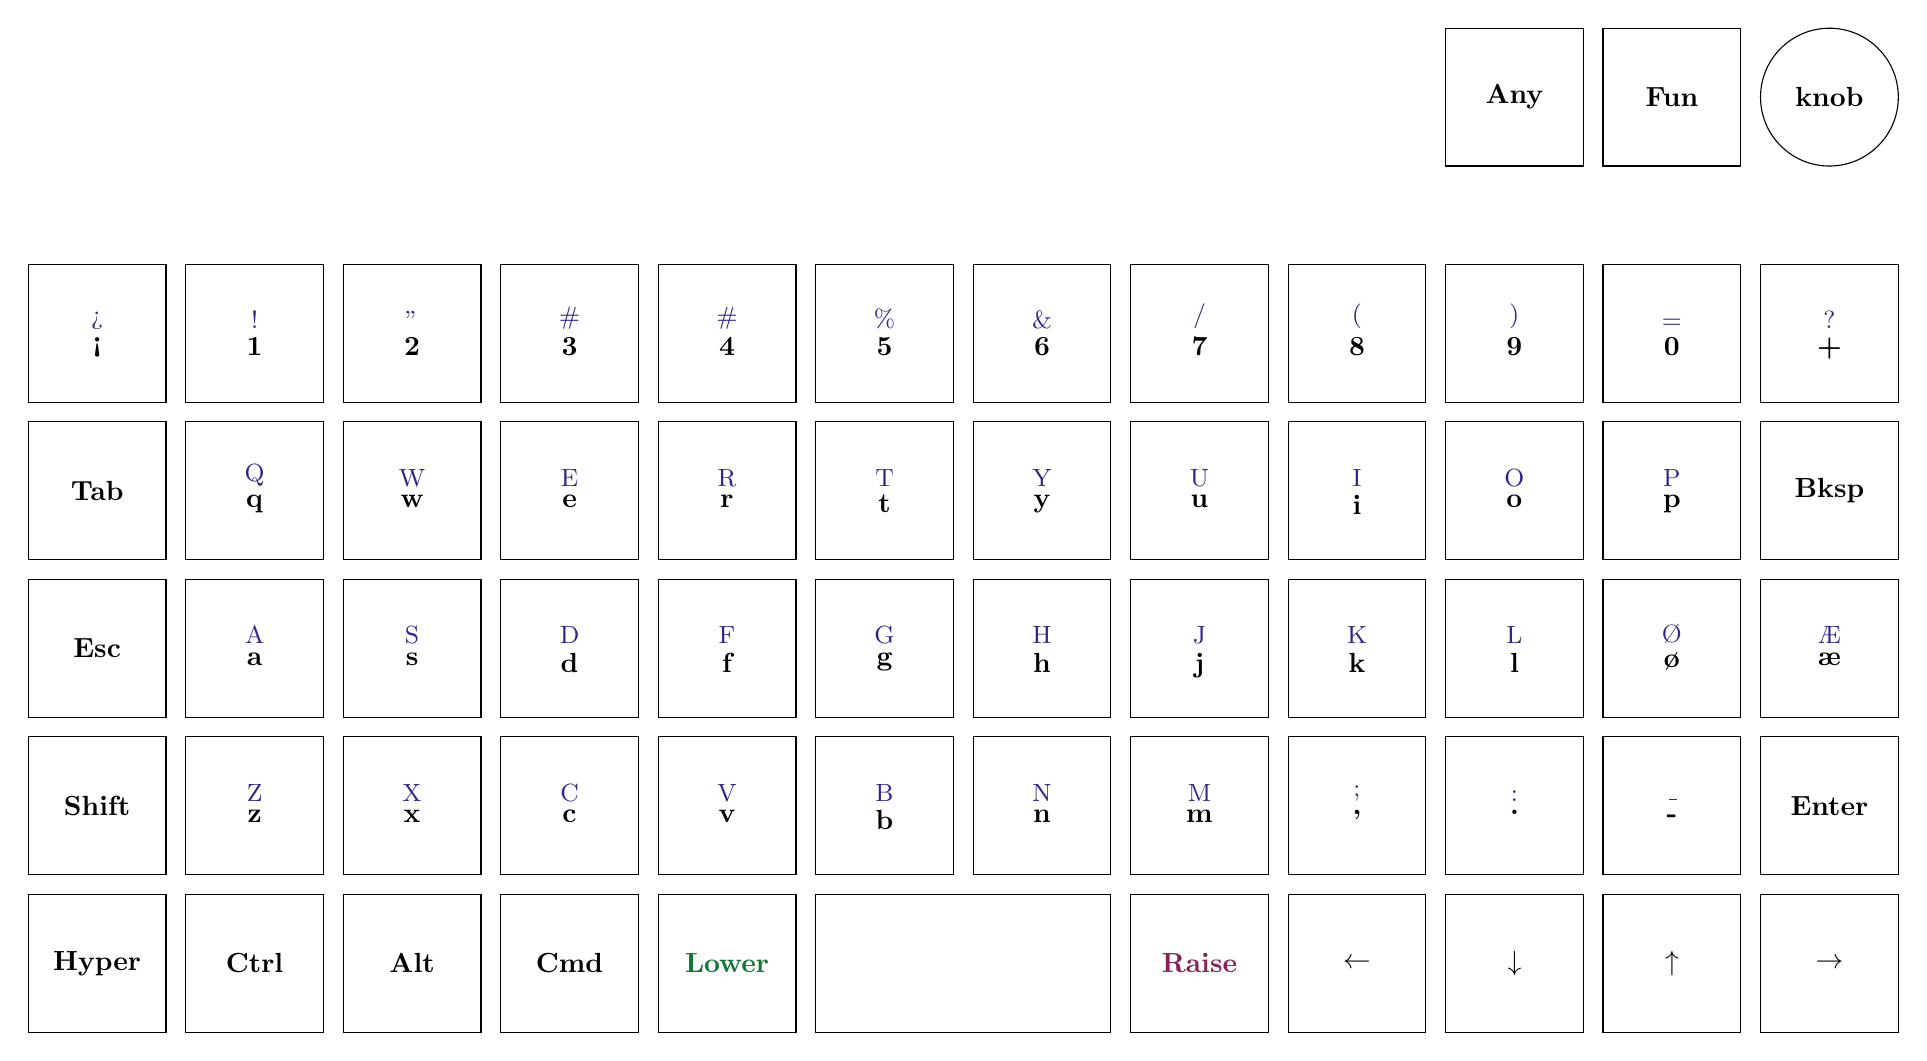
\begin{tikzpicture}[scale=2]
        \node[key] (K0c1) at (9,1.5) {};
        \singleMain{K0c1}{Any}
        \node[key] (K0c2) at (10,1.5) {};
        \singleMain{K0c2}{Fun}<
        \node[knob] (K0c3) at (11,1.5) {};
        \singleMain{K0c3}{knob}
        %
        \node[key] (K1c1) at (0,0) {};
        \main{K1c1}{<}{>}
        \node[key] (K1c2) at (1,0) {};
        \main{K1c2}{1}{!}
        \node[key] (K1c3) at (2,0) {};
        \main{K1c3}{2}{"}
        \node[key] (K1c4) at (3,0) {};
        \main{K1c4}{3}{\#}
        \node[key] (K1c5) at (4,0) {};
        \main{K1c5}{4}{\#}
        \node[key] (K1c6) at (5,0) {};
        \main{K1c6}{5}{\%}
        \node[key] (K1c7) at (6,0) {};
        \main{K1c7}{6}{\&}
        \node[key] (K1c8) at (7,0) {};
        \main{K1c8}{7}{/}
        \node[key] (K1c9) at (8,0) {};
        \main{K1c9}{8}{(}
        \node[key] (K1c10) at (9,0) {};
        \main{K1c10}{9}{)}
        \node[key] (K1c11) at (10,0) {};
        \main{K1c11}{0}{=}
        \node[key] (K1c12) at (11,0) {};
        \main{K1c12}{+}{?}
        %
        %
        % Second line
        \node[key] (K2c1) at (0,-1) {};
        \singleMain{K2c1}{Tab}
        \node[key] (K2c2) at (1,-1) {};
        \main{K2c2}{q}{Q}
        \node[key] (K2c3) at (2,-1) {};
        \main{K2c3}{w}{W}
        \node[key] (K2c4) at (3,-1) {};
        \main{K2c4}{e}{E}
        \node[key] (K2c5) at (4,-1) {};
        \main{K2c5}{r}{R}
        \node[key] (K2c6) at (5,-1) {};
        \main{K2c6}{t}{T}
        \node[key] (K2c7) at (6,-1) {};
        \main{K2c7}{y}{Y}
        \node[key] (K2c8) at (7,-1) {};
        \main{K2c8}{u}{U}
        \node[key] (K2c9) at (8,-1) {};
        \main{K2c9}{i}{I}
        \node[key] (K2c10) at (9,-1) {};
        \main{K2c10}{o}{O}
        \node[key] (K2c11) at (10,-1) {};
        \main{K2c11}{p}{P}
        \node[key] (K2c12) at (11,-1) {};
        \singleMain{K2c12}{Bksp}
        %
        %
        % Third line
        \node[key] (K3c1) at (0,-2) {};
        \singleMain{K3c1}{Esc}
        \node[key] (K3c2) at (1,-2) {};
        \main{K3c2}{a}{A}
        \node[key] (K3c3) at (2,-2) {};
        \main{K3c3}{s}{S}
        \node[key] (K3c4) at (3,-2) {};
        \main{K3c4}{d}{D}
        \node[key] (K3c5) at (4,-2) {};
        \main{K3c5}{f}{F}
        \node[key] (K3c6) at (5,-2) {};
        \main{K3c6}{g}{G}
        \node[key] (K3c7) at (6,-2) {};
        \main{K3c7}{h}{H}
        \node[key] (K3c8) at (7,-2) {};
        \main{K3c8}{j}{J}
        \node[key] (K3c9) at (8,-2) {};
        \main{K3c9}{k}{K}
        \node[key] (K3c10) at (9,-2) {};
        \main{K3c10}{l}{L}
        \node[key] (K3c11) at (10,-2) {};
        \main{K3c11}{ø}{Ø}
        \node[key] (K3c12) at (11,-2) {};
        \main{K3c12}{æ}{Æ}
        %
        %
        % Fourth line
        \node[key] (K4c1) at (0,-3) {};
        \singleMain{K4c1}{Shift}
        \node[key] (K4c2) at (1,-3) {};
        \main{K4c2}{z}{Z}
        \node[key] (K4c3) at (2,-3) {};
        \main{K4c3}{x}{X}
        \node[key] (K4c4) at (3,-3) {};
        \main{K4c4}{c}{C}
        \node[key] (K4c5) at (4,-3) {};
        \main{K4c5}{v}{V}
        \node[key] (K4c6) at (5,-3) {};
        \main{K4c6}{b}{B}
        \node[key] (K4c7) at (6,-3) {};
        \main{K4c7}{n}{N}
        \node[key] (K4c8) at (7,-3) {};
        \main{K4c8}{m}{M}
        \node[key] (K4c9) at (8,-3) {};
        \main{K4c9}{,}{;}
        \node[key] (K4c10) at (9,-3) {};
        \main{K4c10}{.}{:}
        \node[key] (K4c11) at (10,-3) {};
        \main{K4c11}{-}{\_}
        \node[key] (K4c12) at (11,-3) {};
        \singleMain{K4c12}{Enter}
        %
        %
        % Fifth line
        \node[key] (K5c1) at (0,-4) {};
        \singleMain{K5c1}{Hyper}
        \node[key] (K5c2) at (1,-4) {};
        \singleMain{K5c2}{Ctrl}
        \node[key] (K5c3) at (2,-4) {};
        \singleMain{K5c3}{Alt}
        \node[key] (K5c4) at (3,-4) {};
        \singleMain{K5c4}{Cmd}
        \node[key] (K5c5) at (4,-4) {};
        \singleMain{K5c5}{\color{TolMutedGreen} Lower}
        \node[key, minimum width = 3.75cm] (K5c6) at (5.5,-4) {};
        \node[key] (K5c7) at (7,-4) {};
        \singleMain{K5c7}{\color{TolMutedWine} Raise}
        \node[key] (K5c8) at (8,-4) {};
        \singleMain{K5c8}{$\leftarrow$}
        \node[key] (K5c9) at (9,-4) {};
        \singleMain{K5c9}{$\downarrow$}
        \node[key] (K5c10) at (10,-4) {};
        \singleMain{K5c10}{$\uparrow$}
        \node[key] (K5c11) at (11,-4) {};
        \singleMain{K5c11}{$\rightarrow$}
    \end{tikzpicture}
\end{document}